\documentclass[11pt]{article}

% ---------- packages ----------
\usepackage{comment}
\usepackage[T1]{fontenc}
\usepackage[utf8]{inputenc}
\usepackage[a4paper,margin=1in]{geometry}
\emergencystretch=2.5em
\usepackage{xcolor}
\usepackage{listings}
\usepackage{booktabs}
\usepackage{enumitem}
\usepackage{titlesec}
\usepackage{fancyhdr}
\usepackage{tikz}
\usepackage{amssymb}
\usepackage[hidelinks]{hyperref}
\usetikzlibrary{arrows.meta,positioning,fit,backgrounds,calc}

% ---------- colors ----------
\definecolor{accent}{HTML}{1F6FEB}
\definecolor{accentdark}{HTML}{0B3D91}
\definecolor{ink}{HTML}{1A1A1A}
\definecolor{slate}{HTML}{55606E}
\definecolor{codebg}{HTML}{F6F8FA}
\definecolor{codeframe}{HTML}{D0D7DE}
\definecolor{kw}{HTML}{CF222E}
\definecolor{cmt}{HTML}{6E7781}
\definecolor{str}{HTML}{0A3069}
\definecolor{typ}{HTML}{8250DF}
\definecolor{boxbg}{HTML}{EEF4FF}
\definecolor{greenborder}{HTML}{1A7F37}
\definecolor{greenbg}{HTML}{EDF7ED}

% ---------- listings ----------
\lstset{
  language=C++,
  basicstyle=\ttfamily\footnotesize,
  backgroundcolor=\color{codebg},
  frame=single,
  rulecolor=\color{codeframe},
  framesep=6pt,
  xleftmargin=10pt,
  xrightmargin=4pt,
  keywordstyle=\color{kw}\bfseries,
  commentstyle=\color{cmt}\itshape,
  stringstyle=\color{str},
  identifierstyle=\color{ink},
  showstringspaces=false,
  breaklines=true,
  columns=fullflexible,
  keepspaces=true,
  tabsize=2,
  morekeywords={constexpr,noexcept,nullptr,override,final,co_await,
    string_view,size_t,uint64_t,intptr_t,std,atomic,shared_mutex,
    jthread,expected,optional,memory_order_acquire,memory_order_release,
    memory_order_relaxed,memory_order_acq_rel,alignas}
}
\newcommand{\ic}[1]{\lstinline|#1|}

% ---------- section styling ----------
\titleformat{\section}{\Large\bfseries\color{accentdark}}{\thesection}{0.6em}{}
\titleformat{\subsection}{\large\bfseries\color{ink}}{\thesubsection}{0.6em}{}
\titlespacing*{\section}{0pt}{16pt}{6pt}

% ---------- headers ----------
\pagestyle{fancy}
\fancyhf{}
\renewcommand{\headrulewidth}{0.4pt}
\lhead{\small\color{slate}Catalyst Orchestrated Builder}
\rhead{\small\color{slate}Architecture \& Techniques}
\cfoot{\small\color{slate}\thepage}

% ---------- callout box ----------
\newcommand{\callout}[2]{%
  \begin{center}\begin{tikzpicture}
  \node[draw=accent,fill=boxbg,rounded corners,line width=0.8pt,
        inner sep=8pt,text width=0.94\linewidth] {%
    {\color{accentdark}\bfseries #1}\\[2pt]\small #2};
  \end{tikzpicture}\end{center}}

\setlist[itemize]{leftmargin=1.4em,itemsep=2pt,topsep=3pt}

% =====================================================================
\begin{document}

% ---------- title ----------
\begin{titlepage}
\vspace*{2.2cm}
\begin{flushleft}
{\color{accent}\rule{\linewidth}{2pt}}\\[10pt]
{\Huge\bfseries\color{accentdark} Catalyst Orchestrated Builder}\\[8pt]
{\LARGE\color{ink} Architecture and Implementation Techniques}\\[14pt]
{\large\color{slate} A High-Performance Parallel Execution Engine for Low-Level Dependency Graphs in C++23}\\[6pt]
{\color{accent}\rule{\linewidth}{1pt}}
\end{flushleft}

\vfill
\begin{flushleft}
\large
\textbf{Subject:} \texttt{cob} v0.5.0 --- The Catalyst Orchestrated Builder \\[4pt]
\textbf{Author:} Siddharth Mohanty\\
\textbf{Scope:} parser, build graph, execution engine, concurrency, I/O, codegen targets\\[4pt]
\textbf{Language:} C++23 \\[4pt]
\textbf{License:} Apache-2.0\\[14pt]
\textit{\color{slate} A formal architectural analysis of low-overhead parsing, lock-free queue scheduling, and memory-mapped metadata serialization in the Catalyst execution backend.}
\end{flushleft}
\vspace{1cm}
\end{titlepage}

\tableofcontents
\thispagestyle{empty}
\clearpage

% =====================================================================
\section{Overview and Design Invariants}

COB (the \emph{Catalyst Orchestrated Builder}) is a specialized, low-overhead execution
backend for machine-generated build manifests emitted by the Catalyst meta-build
system. Operating in the same structural layer as Ninja beneath CMake or Meson,
COB's architectural boundary separates high-level meta-configuration
(such as profile resolution, compiler toolchain mapping, and dependency
package retrieval) from the mechanical execution of directed acyclic dependency
graphs.

This decoupling is the foundational design constraint of the system. The
meta-build layer processes compiler profiles and emits a flat, pipe-delimited
manifest. Enabling COB to be optimized for a single objective: ingest this
manifest and drive the implied transformations with minimal scheduling overhead,
while enforcing robust incremental rebuilding guarantees.

Three engineering invariants govern the implementation:

\begin{itemize}
  \item \textbf{Zero-copy where possible.} The manifest, dependency files, and
  binary cache are memory-mapped, and nearly every internal string is a
  \lstinline|std::string_view| pointing directly into a mapped region. The
  build graph stores no owned strings for paths or tool names; it borrows from
  files whose lifetime it explicitly extends.
  \item \textbf{Pay parsing cost once.} A text manifest is parsed into a graph,
  then serialized to a platform-tagged binary cache (\texttt{.catalyst.bin}).
  Subsequent invocations bypass text parsing entirely when the cache is newer
  than the manifest.
  \item \textbf{Lock-free on the hot path.} The parallel scheduler coordinates
  worker threads through Vyukov bounded queues and atomic in-degree counters,
  reserving mutexes only for the stat cache, where the critical section is a
  binary search.
\end{itemize}

\callout{Architectural Invariant}
{COB operates strictly as a low-abstraction mechanical execution layer.
By delegating compiler profile resolution and custom macro expansion to the
Catalyst meta-build generator, the executor operates over regular,
pipe-delimited targets, bypassing the computational overhead of generic macro
parsing and variable evaluation loops.}

% =====================================================================
\section{System Architecture}

The execution path is a short, linear pipeline. The CLI parses arguments into an
\lstinline|ExecutorConfig|; the parser populates a \lstinline|COBBuilder|
(either from the binary cache or the text manifest); the builder hands a
finished \lstinline|BuildGraph| to the \lstinline|Executor|, which (optionally
guided by historical execution cost loaded from \texttt{catalyst.estimates})
either runs the parallel build or emits one of several auxiliary artifacts.

\begin{center}
\resizebox{\textwidth}{!}{%
\definecolor{accent}{HTML}{1A73E8}
\definecolor{boxbg}{HTML}{F1F3F4}
\definecolor{slate}{HTML}{5F6368}
\definecolor{codebg}{HTML}{F8F9FA}
\definecolor{greenborder}{HTML}{137333}
\definecolor{greenbg}{HTML}{E6F4EA}
\definecolor{accentdark}{HTML}{1557B0}

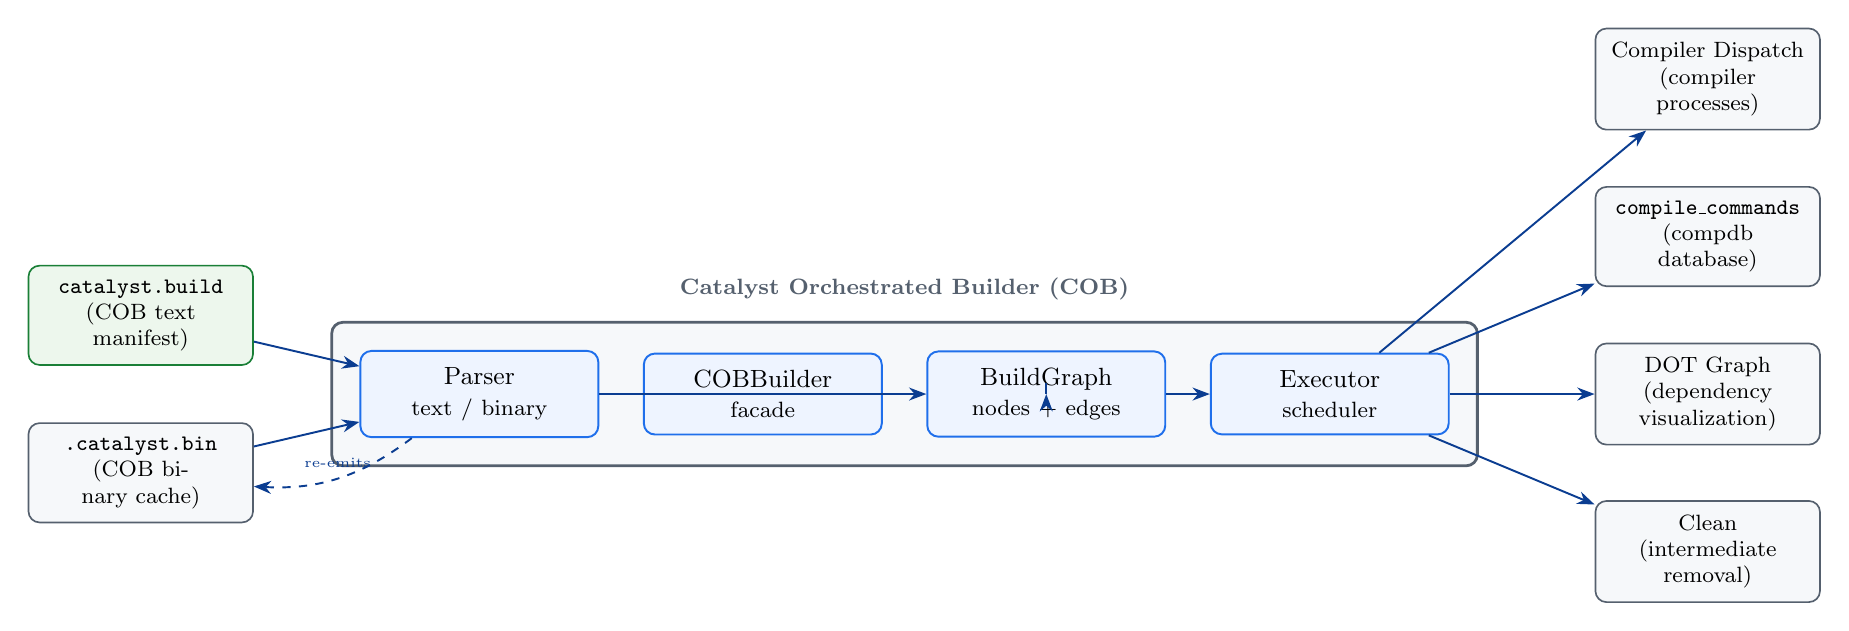
\begin{tikzpicture}[
  font=\small,
  box/.style={draw=accent,fill=boxbg,rounded corners,line width=0.7pt,
    align=center,inner sep=6pt,minimum height=2.2em,text width=2.6cm},
  subc/.style={draw=accent,fill=boxbg,rounded corners,line width=0.6pt,
    align=center,inner sep=4pt,font=\footnotesize\ttfamily,minimum height=1.6em,text width=2.0cm},
  io/.style={draw=slate,fill=codebg,rounded corners,line width=0.6pt,
    align=center,inner sep=5pt,text width=2.5cm,font=\footnotesize},
  greenio/.style={draw=greenborder,fill=greenbg,rounded corners,line width=0.6pt,
    align=center,inner sep=5pt,text width=2.5cm,font=\footnotesize},
  ar/.style={-{Stealth[length=2.2mm]},line width=0.7pt,accentdark}
]

\node[greenio] (cob_file) at (0.0, 1.0) {\texttt{catalyst.build}\\\footnotesize(COB text manifest)};
\node[io] (cob_bin) at (0.0, -1.0) {\texttt{.catalyst.bin}\\\footnotesize(COB binary cache)};

\node[box] (cob_parse) at (4.3, 0.0) {Parser\\\footnotesize text / binary};
\node[box] (cob_builder) at (7.9, 0.0) {COBBuilder\\\footnotesize facade};
\node[box] (cob_builder) at (11.5, 0.0) {BuildGraph\\\footnotesize nodes + edges};
\node[box] (cob_exec) at (15.1, 0.0) {Executor\\\footnotesize scheduler};

\draw[ar] (cob_file) -- (cob_parse);
\draw[ar] (cob_bin) -- (cob_parse);
\draw[ar, dashed, bend left=20] (cob_parse) to node[above, font=\tiny] {re-emits} (cob_bin);
\draw[ar] (cob_parse) -- (cob_builder);
\draw[ar] (cob_builder) -- (cob_builder);
\draw[ar] (cob_builder) -- (cob_exec);

\begin{scope}[on background layer]
  \node[draw=slate, line width=1.0pt, rounded corners, fill=codebg,
        fit=(cob_parse)(cob_exec), inner sep=10pt] (cob_group) {};
\end{scope}
\node[slate, font=\footnotesize\bfseries, above=4pt of cob_group] (cob_title) {Catalyst Orchestrated Builder (COB)};

% ==================== 3. OUTPUTS & BACKENDS ====================
\node[io] (out1) at (19.9, 4.0) {Compiler Dispatch\\\footnotesize(compiler processes)};
\node[io] (out2) at (19.9, 2.0) {\texttt{compile\_commands}\\\footnotesize(compdb database)};
\node[io] (out3) at (19.9, 0.0) {DOT Graph\\\footnotesize(dependency visualization)};
\node[io] (out4) at (19.9, -2.0) {Clean\\\footnotesize(intermediate removal)};

\draw[ar] (cob_exec) -- (out1);
\draw[ar] (cob_exec) -- (out2);
\draw[ar] (cob_exec) -- (out3);
\draw[ar] (cob_exec) -- (out4);

\end{tikzpicture}
}
\end{center}

As illustrated in the toolchain diagram, COB operates within the broader \textbf{Catalyst Toolchain} ecosystem.
The input manifest \texttt{catalyst.build} is generated directly by the \textbf{Catalyst Build System}.
On the first pass of a modified manifest, the COB Parser parses the text representation and serializes it into the
binary cache \texttt{.catalyst.bin} (re-emitting it for subsequent fast-path loads).
Meanwhile, LPT task-scheduling metrics are fed from the \texttt{catalyst.estimates} file, which is maintained and
updated by \textbf{catalyst ccache} to store historical compilation costs. During compiler dispatch, the actual compilation
statistics are fed back into \textbf{catalyst ccache} to record and refine future task estimates. Additionally, because
COB operates on a simple, low-abstraction text manifest, alternative generators (\textbf{Other Meta Build Systems}
like CMake or custom wrappers) can also emit the \texttt{catalyst.build} manifest
to leverage COB's high-performance parallel execution engine.

The translation units map cleanly onto these stages. \texttt{cli\_args.cpp}
produces the configuration; \texttt{parser.cpp} and \texttt{binary.cpp} feed the
builder; \texttt{graph.cpp} owns the dependency representation;
\texttt{executor.cpp} (with \texttt{executor\_stat\_cache.cpp},
\texttt{process\_exec.cpp}, \texttt{json.cpp}, and \texttt{work\_estimate.cpp})
implements scheduling and side effects. The header
\texttt{cob/utility.hpp} establishes the error-handling vocabulary for the whole
project in a single line:

\begin{lstlisting}
template <typename Value_T>
using Result = std::expected<Value_T, std::string>;
\end{lstlisting}

Every fallible operation returns \lstinline|Result<Value_T>|, and errors propagate as
human-readable strings via \lstinline|std::unexpected|. There are no exceptions
on the control path except where the OS mapping layer throws, which is caught
and converted to a \lstinline|Result| at the boundary.

% =====================================================================
\section{The Data Model}

\subsection{Build steps and definitions}

The atomic unit of work is the \lstinline|BuildStep| (\texttt{build\_step.hpp}).
It describes a single transformation: a \emph{tool} (\texttt{cc}, \texttt{cxx},
\texttt{ld}, \texttt{ar}, \texttt{sld}) applied to a set of \emph{inputs} to
produce one \emph{output}.

\begin{lstlisting}
struct BuildStep {
    std::string_view tool;
    std::string_view inputs;   // raw, comma-separated
    std::string_view output;
    catalyst::optional_vector<std::string_view> opaque_inputs;
    catalyst::optional_vector<std::string_view> depfile_inputs;
    std::vector<std::string_view> parsed_inputs;
};
\end{lstlisting}

The distinction between the three input kinds is the heart of COB's
dependency model:

\begin{itemize}
  \item \textbf{Parsed inputs} are the explicit sources listed in the manifest.
  \item \textbf{Opaque inputs} are implicit or order-only dependencies that
  affect the build but are not passed on the command line --- they are written
  in the manifest with a leading \lstinline|!|
  (e.g.\ \lstinline|input.c,!opaque.txt|).
  They participate in rebuild decisions but never appear in the compiler
  invocation.
  \item \textbf{Depfile inputs} are discovered dynamically by parsing the
  \texttt{.d} sidecar files that Clang/GCC emit (header dependencies).
\end{itemize}

Global variables, compiler paths and flags, live in an associative
\lstinline|Definitions| map (with a future transition to a cache-friendly sorted flat map planned), again keyed and
valued by views. While the keys in the definitions map can be any arbitrary string, only specific toolchain variables
are respected and utilized by the build execution engine: \texttt{cc}, \texttt{cxx}, \texttt{linker}, \texttt{archiver}, \texttt{cxxflags}, \texttt{cflags}, \texttt{ldflags}, and \texttt{ldlibs}.

\begin{lstlisting}
using Definitions = std::flat_map<std::string_view, std::string_view>;
\end{lstlisting}

\subsection{Borrowed strings and resource lifetime}

Because paths and flags are all \lstinline|string_view|s into mapped files, the
graph must keep those files alive for as long as any view into them is reachable.
This is handled by a type-erased resource list. \lstinline|COBBuilder| and
\lstinline|BuildGraph| hold \lstinline|std::vector<std::shared_ptr<void>>|, and
every mapped file is registered via \lstinline|add_resource|:

\begin{lstlisting}
void add_resource(std::shared_ptr<void> res) {
    resources_.emplace_back(std::move(res));
}
\end{lstlisting}

The \lstinline|shared_ptr<void>| erases the concrete type (it may be a
\lstinline|MappedFile| or a \lstinline|MappedUnfaultedFile|) while still running
the correct destructor, because the deleter is captured at construction. This is
the idiomatic way to attach arbitrary keep-alive resources to an owner without
templating the owner on every resource type. It trades a small amount of
control-block overhead for the elimination of per-string allocation across the
entire graph.

% =====================================================================
\section{Parsing}

\subsection{The text manifest format}

The manifest is line-oriented and pipe-delimited. By stripping away
conventional syntax boilerplate, the design achieves a highly minimal, format
that is also trivially fast for the machine to parse, conforming to the following
schema:

\begin{lstlisting}[language=,basicstyle=\ttfamily\fontsize{7}{7}\selectfont]
Manifest:
      (Line EOL)*
Line:
      Comment
      Definition
      BuildStep
      Empty
Comment:
      '#' String
Definition:
      'DEF' '|' Key '|' Value
BuildStep:
      Tool '|' Inputs '|' Output
Empty:
      <empty>
Inputs:
      (Input (',' Input)*)?
Input:
      ParsedInput
      OpaqueInput
ParsedInput:
      Path
OpaqueInput:
      '!' Path
EOL:
      '\r'? '\n'
Key:
      'archiver'
      'cc'
      'cflags'
      'cxx'
      'cxxflags'
      'ldflags'
      'ldlibs'
      'linker'
      [^|\r\n]*
Tool:
      'ar'
      'cc'
      'cxx'
      'ld'
      'sld'
Value, Output, String:
      [^\r\n]*
Path:
      [^,|\r\n]+
\end{lstlisting}

Parsing (\texttt{parser.cpp}) walks the mapped buffer with
\lstinline|find('\n')|, strips a trailing \lstinline|\r| for Windows CRLF
tolerance, and dispatches on the line prefix. The two pipe positions are located
with \lstinline@find('|')@ and the fields are taken as substrings without
intermediate tokenization or memory allocation. Because the producer is trusted,
malformed lines yield an error rather than recovery. Although the parser permits
any arbitrary string as a \texttt{Key} for the sake of future extensibility,
the execution engine strictly respects only a pre-defined set of variables:
\texttt{cc}, \texttt{cxx}, \texttt{linker}, \texttt{archiver},
\texttt{cxxflags}, \texttt{cflags}, \texttt{ldflags}, and \texttt{ldlibs}.

\subsection{Dependency files}

Header dependencies come from the Make-style \texttt{.d} files generated by the
compiler. \texttt{graph.cpp} contains a small hand-written depfile parser that
correctly handles the awkward features of that format: backslash line
continuations, backslash-escaped spaces in paths, and the handling of colons. The presence of colons is notoriously a relic of Windows drive-letter support, requiring parsers to differentiate drive letters (like \texttt{C:}) from target-dependency separators. The parser scans with
\lstinline|memchr| to isolate the separating \lstinline|:| separating target from
prerequisites, then alternates \lstinline|skipWhitespace| and
\lstinline|extractToken| over the remainder, invoking a callback per
dependency. The depfile is mapped through \lstinline|MappedUnfaultedFile| ---
it is read exactly once, so prefaulting its pages would be wasted work (see
\S\ref{sec:mmap}).

The GCC/Clang Makefile-style dependency files conform to the following language schema:

\begin{lstlisting}[language=,basicstyle=\ttfamily\fontsize{7}{7}\selectfont]
Depfile:
      Target ':' Dependents
Target:
      Path
Dependents:
      (Separator Path)* Separator?
Separator:
      Whitespace
      Continuation
Continuation:
      '\' EOL Whitespace*
Whitespace:
      [ \t]+
EOL:
      '\r'? '\n'
Path:
      (EscapedSpace | [^\\\s:\r\n])+
EscapedSpace:
      '\' ' '
\end{lstlisting}

Below is an example of a generated \texttt{.d} file:

\begin{lstlisting}[language=,basicstyle=\ttfamily\fontsize{7}{7}\selectfont]
obj/binary_7d9517a626d9ccfc.o: \
  /home/user/project/src/binary.cpp \
  /home/user/project/include/cob/binary.hpp \
  /home/user/project/include/cob/builder.hpp \
  /home/user/project/include/cob/graph.hpp \
  /home/user/project/include/cob/build_step.hpp \
  /home/user/project/include/cob/optional_vector.hpp \
  /home/user/project/include/cob/utility.hpp \
  /home/user/project/include/cob/file_handle.hpp
\end{lstlisting}

\subsection{Binary Caches}

The most consequential parsing optimization is the binary cache. After a
successful text parse, \lstinline|emit_bin| serializes the entire graph to
\texttt{.catalyst.bin}; on the next run, \lstinline|parse| checks the cache's
timestamp against the manifest and, if newer, calls \lstinline|parse_bin| to
reconstruct the graph directly:

\begin{lstlisting}
if (std::filesystem::exists(".catalyst.bin") &&
    std::filesystem::last_write_time(".catalyst.bin") >
        std::filesystem::last_write_time(path)) {
    return parse_bin(builder);
}
\end{lstlisting}

The on-disk layout is a fixed header followed by definitions, nodes, and steps,
with a \emph{string table} appended at the end of the file. Alongside strings and structural fields, each step serializes a 64-bit FNV-1a hash of its exact command-line invocation (\lstinline|command_hash|). This hash persists across runs, allowing the execution engine to quickly determine if compiler flags or arguments changed between builds, invalidating the step even if timestamps match. All string-bearing
fields are stored as \lstinline|StringRef{offset, len}| pairs that index into
that table. During serialization a \lstinline|StringBuffer| interns strings ---
identical views collapse to a single entry via a custom
\lstinline|catalsyt::FlatHashMap<string_view, StringRef>| cache --- so the table is
deduplicated. On load, the file is mapped, the header is
\lstinline|reinterpret_cast| in place, and a closure resolves each
\lstinline|StringRef| against the string base:

\begin{lstlisting}
auto get_sv = [&](StringRef ref) -> std::string_view {
    return {strings_base + ref.offset, ref.len};
};
\end{lstlisting}

Because views point straight into the mapped cache, loading is effectively a
pointer-arithmetic pass with no string copies. The header magic is
platform-tagged (\texttt{CATBL\#\#\#} on Linux, \texttt{CATBM\#\#\#} on macOS, and \texttt{CATBW\#\#\#} on Windows) so
a cache produced on one platform is rejected rather than misinterpreted on
another.

\callout{Why a string table?}{Storing every string once and referencing it by
\texttt{(offset, len)} keeps the binary compact, makes the load a single linear
read, and --- crucially --- preserves the zero-copy invariant: the
deserialized graph borrows from the mapped cache exactly as the parsed graph
borrowed from the mapped manifest.}

% =====================================================================
\section{The Build Graph}

\lstinline|BuildGraph| (\texttt{graph.hpp}) is a directed acyclic graph of file
nodes. Each \lstinline|Node| stores its path, a list of \emph{out-edges}
(indices of nodes that depend on it), and an optional \lstinline|step_id|
identifying the step that produces it. Nodes are deduplicated through an
index map so that a file referenced as both an output of one step and an input
of another resolves to a single node:

\begin{lstlisting}
size_t BuildGraph::get_or_create_node(std::string_view path) {
    if (auto it = index_.find(path); it != index_.end())
        return it->second;
    size_t id = nodes_.size();
    nodes_.push_back({path, {}, std::nullopt});
    index_.emplace(path, id);
    return id;
}
\end{lstlisting}

\lstinline|add_step| performs the comma-split of the raw \lstinline|inputs|
string, routing \lstinline|!|-prefixed entries into \lstinline|opaque_inputs|
and the rest into \lstinline|parsed_inputs|, then wires an edge from every input
node to the output node. For compile steps it additionally parses the
\texttt{.d} file (if present) and records each discovered header as both a graph
edge and a depfile input. A duplicate producer for a single output is rejected
as an error.

Ordering is established by a depth-first topological sort with three-color cycle
detection:

\begin{lstlisting}
enum class STATUS : uint8_t { UNSTARTED, WORKING, FINISHED };
// ... a node re-entered while WORKING indicates a cycle:
else if (status[v] == STATUS::WORKING)
    return std::unexpected(std::format(
        "Cycle detected in the build graph at: {}", nodes_[v].path));
\end{lstlisting}

The topological order is used directly by the artifact emitters
(\texttt{compdb}, \texttt{commands}); the parallel executor instead derives its
schedule from in-degree counts, which gives equivalent ordering guarantees
without forcing a serial sequence (\S\ref{sec:exec}).

% =====================================================================
\section{Memory-Mapped I/O}\label{sec:mmap}

All file ingestion goes through \lstinline|MappedFile| (\texttt{file\_handle.hpp}),
a cross-platform RAII wrapper over \lstinline|mmap| (POSIX) and
\lstinline|CreateFileMapping|/\lstinline|MapViewOfFile| (Windows). Empty files
are handled as a special case (no mapping, null data, empty
\lstinline|content()|), and the destructor unmaps and closes unconditionally.

The notable technique here is \textbf{prefault control}. On Linux the
constructor takes a \lstinline|populate| flag and selects the mapping flags
accordingly, and it also advises the kernel about the access pattern:

\begin{lstlisting}
posix_fadvise(file_descriptor, 0, 0, POSIX_FADV_SEQUENTIAL);
int flags = populate ? (MAP_POPULATE | MAP_PRIVATE) : MAP_PRIVATE;
void *addr = mmap(nullptr, file_size, PROT_READ, flags, file_descriptor, 0);
\end{lstlisting}

\lstinline|MAP_POPULATE| eagerly faults the whole file into the page cache at
map time, which is the right tradeoff for the manifest and the binary cache:
they are read densely and immediately, so paying the fault cost up front avoids
a storm of minor page faults during parsing. The dedicated subclass
\lstinline|MappedUnfaultedFile| flips \lstinline|populate| to \lstinline|false|
and is used for \texttt{.d} depfiles, which are short and read once --- there is
nothing to amortize, so lazy faulting is cheaper. This is a deliberate
per-call-site policy rather than a global default.

% =====================================================================
\section{The Execution Engine}\label{sec:exec}

The \lstinline|Executor| subsystem implements a parallel, dependency-aware walk
of the directed acyclic graph across a thread pool of \lstinline|std::jthread|
workers. Task synchronization and thread coordination are driven by lock-free
atomics and portably implement thread suspension on top of native platform
primitives.

\subsection{Scheduling model}

Rather than executing the topological order serially, the executor uses a
\textbf{Kahn-style in-degree scheme}. Each node's in-degree (number of
unsatisfied dependencies) is held in a \lstinline|std::vector<std::atomic<int>>|.
Nodes that start at in-degree zero are seeded into a ready queue. When a worker
finishes a node, it decrements the in-degree of each dependent; the worker that
drives a dependent's count to zero is the one that enqueues it:

\begin{lstlisting}
for (size_t neighbor : node.out_edges) {
    if (ctx.in_degrees[neighbor].fetch_sub(1, std::memory_order_acq_rel) == 1) {
        push_ready(neighbor, ctx);
    }
}
\end{lstlisting}

The \lstinline|fetch_sub| returning \lstinline|1| means this thread observed the
transition $1\rightarrow 0$, so exactly one thread enqueues each node --- no lock,
no double scheduling.

\subsection{Longest-processing-time ordering}

When work estimates are available, the initial ready set is sorted in
\emph{descending} estimated cost before being enqueued:

\begin{lstlisting}
std::ranges::sort(initial_tasks, [](const auto &a, const auto &b) {
    return a.estimate > b.estimate;
});
\end{lstlisting}

This is the classic \emph{Longest Processing Time first} (LPT) heuristic for
multiprocessor scheduling: dispatching the heaviest jobs first reduces the
makespan tail, since small jobs can fill the gaps left by large ones rather than
the reverse. The per-node estimates come from a separate file consulted via
\lstinline|WorkEstimate::getWorkEstimate| (\S\ref{sec:estimate}).

\subsection{Sleeping, waking, and stall detection}

To minimize CPU consumption, threads undergo futex-backed suspension when
ready queues deplete. The coordinator distinguishes between transient queue
depletion (active processes are still executing in-flight tasks) and terminal
cycle starvation/deadlocks using atomic reference counts:

\begin{lstlisting}
size_t sleeping = ctx.sleeping_threads.fetch_add(1, ...) + 1;
if (sleeping == thread_count &&
    ctx.tasks_available.load(std::memory_order_acquire) == 0) {
    // Every worker is asleep with no tasks: stall / completion race.
    ctx.tasks_available.store(SIZE_MAX, std::memory_order_release);
    ctx.tasks_available.notify_all();
}
\end{lstlisting}

Under a terminal starvation condition, the coordinating worker updates \lstinline|tasks_available| to a sentinel value (\lstinline|std::numeric_limits<size_t>::max()|) and issues a global broadcast. Upon waking, all threads immediately abort, transferring control back to the main thread. A post-execution assertion (\lstinline|completed_count == total_nodes|) guarantees that no unvisited nodes remain in the build graph, serving as a dynamic safety barrier against runtime cycle injections.

\subsection{Per-tool command construction}

\lstinline|build_command_args| translates a step into an \lstinline|argv|
vector, switching on the tool. Compile steps inject \lstinline|-MMD -MF out.d -c|
so the depfile gets regenerated on every compile. The linking path has a
notable robustness feature: when an \lstinline|ld| step has more inputs than a
tunable threshold (50), it writes a \emph{response file} and passes
\lstinline|@out.rsp| instead of expanding every object on the command line:

\begin{lstlisting}
} else if (inputs.size() > TUNABLE_INPUT_SZ) {
    use_rsp = true;
    // ... write one input path per line into out.rsp
}
if (use_rsp) args.push_back(std::string("@") + rsp_path.string());
\end{lstlisting}

This sidesteps the OS command-line length limit (\texttt{ARG\_MAX}) that large
links routinely hit, and the \texttt{.rsp} is reused if it is newer than the
manifest.

\subsection{Incremental rebuild decision}

\lstinline|needs_rebuild| is the freshness check. To verify if a step must run, the executor first generates the expected command-line arguments for the invocation and computes their 64-bit FNV-1a hash. This value is compared against the step's cached \lstinline|command_hash|:
\begin{lstlisting}[language=C++]
if (step.command_hash != current_hash) {
    return true;
}
\end{lstlisting}
This immediately catches flag modifications (e.g., changing \lstinline|-O2| to \lstinline|-O3| or modifying include search paths) even if all input file timestamps are unchanged.

If the command hash matches, the executor checks if the output file is missing, or if the manifest itself, any parsed input, any depfile header, or any opaque dependency is at least as new as the output. Timestamp lookups are funneled through the \lstinline|StatCache| (\S\ref{sec:statcache}) to avoid repeated \lstinline|stat| calls on shared headers. Notably, the manifest itself acts as a dependency of every step, ensuring that structural alterations always trigger correct invalidations.

% =====================================================================
\section{Concurrency Primitives}

\subsection{Vyukov bounded queues}

The ready queue and the progress queue are lock-free bounded ring buffers based
on Dmitry Vyukov's well-known algorithm (\texttt{mpmc\_queue.hpp},
\texttt{mpsc\_queue.hpp}). Each cell carries a sequence number; producers and
consumers advance their positions with \lstinline|compare_exchange_weak| and use
the sequence to detect full/empty without ever taking a lock. Capacity is
rounded up to a power of two with \lstinline|std::bit_ceil| so the modulo
becomes a bitmask:

\begin{lstlisting}
size_t cap = std::bit_ceil(capacity);
buffer_mask_ = cap - 1;
// ... index with (pos & buffer_mask_)
\end{lstlisting}

False sharing is attacked explicitly: the buffer pointer and the two position
counters are each \lstinline|alignas(64)| (a cache line apart), so producers
hammering \lstinline|enqueue_pos_| do not invalidate the cache line holding
\lstinline|dequeue_pos_|.

\subsection{MPSC specialization}

The progress/logging channel has many producers (every worker) but a single
consumer (the dedicated progress thread). The MPSC queue exploits this: the
consumer's \lstinline|dequeue_pos_| is a plain \lstinline|size_t|, not an atomic,
because only one thread ever touches it. This removes a redundant atomic
read-modify-write from every log dequeue --- a small but principled
specialization of the general MPMC structure.

\subsection{The progress thread}

Console and log output are funneled to one thread to keep terminal writes
serialized and off the workers' critical path. Workers enqueue
\lstinline|LogEvent|s and bump a \lstinline|messages_enqueued| counter that the
progress thread waits on. Shutdown uses a \emph{poison pill}: after the pool
joins, the main thread enqueues a final event with
\lstinline|is_poison_pill = true|, and the progress thread returns on seeing it.
This is a clean alternative to a separate ``done'' flag plus a wakeup.

\subsection{Optional heterogeneous-core hinting}

On linux, behind the \lstinline|heterogenous_core_affinity| feature flag, the worker biases
scheduling for hybrid (P-core/E-core) CPUs: before running a step whose estimate
exceeds a threshold it lowers its niceness (a hint toward a performance core) and
restores it afterward. It is a hint via \lstinline|setpriority|, not a hard
affinity pin, which keeps it portable and non-fatal where it has no effect.
\begin{lstlisting}
    // static constexpr size_t TUNABLE_HEAVY_THRESHOLD = ...;
    if (task.estimate > TUNABLE_HEAVY_THRESHOLD) {
        setpriority(PRIO_PROCESS, 0, -5); // Hint: P-core
    } else {
        setpriority(PRIO_PROCESS, 0, 5); // Hint: E-core
    }
\end{lstlisting}

% =====================================================================
\section{Stat Cache}\label{sec:statcache}

A single header may be a prerequisite of dozens of objects; naively each step
would \lstinline|stat| it again. \lstinline|StatCache|
(\texttt{executor\_stat\_cache.cpp}) memoizes modification times in a sorted
vector guarded by a \lstinline|std::shared_mutex|, with a read-then-upgrade
pattern:

\begin{lstlisting}
{   std::shared_lock read_lock(cache_mtx);
    auto it = std::ranges::lower_bound(cache, p, {}, &Entry::path);
    if (it != cache.end() && it->path == p) return {it->time, it->ec};
}
std::lock_guard write_lock(cache_mtx);   // miss: take the write lock
// ... stat once, insert in sorted position
\end{lstlisting}

Readers share the lock; only a miss escalates to exclusive access to perform the
\lstinline|stat| and an ordered insert (the cache stays sorted so the
\lstinline|lower_bound| binary search remains valid). It is the one place COB
chooses a mutex over atomics, because the protected operation --- a binary
search plus occasional insert --- does not map cleanly onto a lock-free
structure.

% =====================================================================
\section{Output Generation}

Beyond building, the executor emits three developer-facing artifacts from the
same graph:

\begin{itemize}
  \item \textbf{\texttt{compile\_commands.json}} (\lstinline|emit_compdb|): a
  compilation database for clangd/IDE tooling, built per compile step in
  topological order. COB ships its own minimal JSON value type
  (\texttt{json.hpp}) backed by a \lstinline|std::flat_map| for objects, plus a
  hand-rolled serializer with proper string escaping (control characters become
  \lstinline|\uXXXX|).
  \item \textbf{Graphviz DOT} (\lstinline|emit_graph|): the dependency graph
  rendered for inspection, with nodes that need rebuilding colored green ---
  a quick visual of what an incremental build would touch.
  \item \textbf{Command listing} (\lstinline|emit_commands|): the exact commands
  that would run, for debugging the toolchain wiring.
\end{itemize}

\subsection{Subprocess execution}

All external invocations route through \lstinline|process_exec|
(\texttt{process\_exec.cpp}), a thin wrapper over the \texttt{reproc++} library.
It supports optional output capture (pipe vs.\ inherit-parent redirection),
working-directory override, and environment extension, returning the
\lstinline|(exit_code, captured_output)| pair inside a \lstinline|Result|.
Capture is enabled only when logging to a file is requested, so the common case
inherits the parent's stdio with no piping overhead.

% =====================================================================
\section{Work Estimation}\label{sec:estimate}

The LPT scheduler is fed by \lstinline|WorkEstimate|
(\texttt{work\_estimate.cpp}), itself a feature-gated module. It maps an
estimates file of \lstinline|path|\,\lstinline=|=\,\textit{integer} lines into a
sorted vector and answers \lstinline|getWorkEstimate(path)| with a
\lstinline|lower_bound| binary search and a \lstinline|std::from_chars| parse of
the value. The lookup is marked \lstinline|[[clang::always_inline]]| because it
sits on the enqueue path. Per the project's configuration, these estimates are
maintained as an exponential moving average of observed step durations, so the
schedule self-tunes across builds: steps that were historically expensive get
dispatched first.

% =====================================================================
\section{Configurability and Self-Hosting}

\subsection{Compile-time feature flags}

COB is aggressively feature-gated through \lstinline|FF_cob__*| preprocessor
macros: \lstinline|binary| (the cache), \lstinline|estimates| (LPT scheduling),
\lstinline|logging| (capture + log file), \lstinline|profiling| (per-step
timing), and \lstinline|heterogenous_core_affinity|. Disabled features compile
out entirely --- the \lstinline|ExecutorConfig| does not even carry an
\lstinline|estimates_file| field unless estimates are enabled. This keeps the
default binary lean and the hot paths free of dead branches.

\subsection{COB builds COB}

The \texttt{CATALYST.yaml} manifest shows the project is self-hosting: it is
built by Catalyst itself. The configuration defines layered profiles ---
\texttt{common}, \texttt{test}, \texttt{benchmark}, \texttt{ccache}, and
\texttt{release} --- that compose tooling and flags. The \texttt{release} profile
is a study in linker tuning: static linking with \texttt{mold}, full LTO,
identical-code folding (\lstinline|--icf=safe|), section garbage collection,
RELRO hardening, and a stripped, reproducible build-id binary. A post-build hook
packs the result. The \texttt{benchmark} profile drops to \lstinline|-O0 -g -fno-omit-frame-pointer| for clean profiles, and \texttt{ccache} simply injects
compiler launchers.

% =====================================================================
\section{Performance Evaluation and Empirical Benchmarks}

To quantitatively evaluate the architectural efficiency of COB, comparative benchmarks were executed against GNU Make (v4.3) and Ninja (v1.11.1) on a high-density mock repository (\texttt{heavy\_repo}) designed to simulate a massive C++ codebase. The workload consists of 1,000 translation units arranged in a balanced binary tree dependency topology to maximize scheduler breadth and depth.

All benchmarks were captured using \texttt{hyperfine} with 2 warmup runs.
The tests were performed on an Intel Core i9 14900KS (8 performance cores, 16 efficiency cores, 32 hardware threads)
running Linux Kernel 7.0.0-15 on Ubuntu 26.04.

\subsection{Full Incremental Build Execution}

The primary benchmark measures the makespan of a full incremental build loop, wherein a clean workspace is built from scratch. For this comparison, GNU Make and Ninja were executed with maximum parallel job parameters matching the hardware capabilities (\texttt{-j32}), while COB utilized its default automated core-detection scheduler.

\begin{center}
\renewcommand{\arraystretch}{1.2}
\begin{tabular}{@{}lcccc@{}}
\toprule
\textbf{Orchestrator} & \textbf{Mean [s]} & \textbf{Min [s]} & \textbf{Max [s]} & \textbf{Relative Performance} \\
\midrule
\texttt{cob}   & $1.623 \pm 0.040$ & $1.555$ & $1.714$ & $1.00$ \\
\texttt{ninja} & $1.833 \pm 0.017$ & $1.813$ & $1.870$ & $1.13 \pm 0.03$ \\
\texttt{make}  & $2.217 \pm 0.015$ & $2.198$ & $2.245$ & $1.37 \pm 0.04$ \\
\bottomrule
\end{tabular}
\end{center}

COB achieves a statistically significant 13\% speedup over Ninja and a 37\% speedup over GNU Make.
This acceleration is driven by three architectural vectors:
\begin{enumerate}
    \item \textbf{Binary Serialization Warm Path}: COB bypasses text-based parsing of the build manifest on subsequent runs, loading the pre-compiled \texttt{.catalyst.bin} via in-place \lstinline|reinterpret_cast| pointers on memory-mapped pages.
    \item \textbf{High-Efficiency Lock-Free Scheduling}: Coordination between worker threads utilizes Dmitry Vyukov MPMC queues and atomic in-degree decrements. In contrast, Ninja relies on lock-heavy scheduling queues and serial state checks, which induce cacheline bouncing and lock contention at high thread counts (32 threads).
    \item \textbf{Longest Processing Time (LPT) Ordering}: Pre-sorting root tasks based on Exponential Moving Average (EMA) historical execution estimates ensures that compiler bottlenecks are scheduled early, minimizing the tail execution makespan.
\end{enumerate}

\subsection{Workspace Cleanup and CompDB Generation}

To ensure complete transparency and prevent overstating COB's performance profile, secondary tasks were benchmarked
to identify overhead profiles. These tasks do not run compiler processes and are governed entirely by metadata
read/write performance.

\begin{center}
\renewcommand{\arraystretch}{1.2}
\begin{tabular}{@{}lcccc@{}}
\toprule
\textbf{Operation / Command} & \textbf{Mean [ms]} & \textbf{Min [ms]} & \textbf{Max [ms]} & \textbf{Relative} \\
\midrule
\textbf{Clean Subcommand} & & & & \\
\quad\texttt{ninja -t clean} & $11.7 \pm 2.2$ & $9.8$ & $16.0$ & $1.00$ \\
\quad\texttt{cob -t clean}   & $15.9 \pm 1.7$ & $14.5$ & $20.4$ & $1.37 \pm 0.30$ \\
\quad\texttt{make clean}      & $351.9 \pm 14.0$ & $334.9$ & $373.9$ & $30.21 \pm 5.86$ \\
\midrule
\textbf{CompDB Generation} & & & & \\
\quad\texttt{cob -t compdb}   & $3.5 \pm 0.4$ & $2.3$ & $4.5$ & $1.00$ \\
\quad\texttt{ninja -t compdb} & $4.5 \pm 0.7$ & $3.1$ & $5.7$ & $1.28 \pm 0.24$ \\
\bottomrule
\end{tabular}
\end{center}

COB exhibits highly competitive performance profiles on purely metadata-driven tasks, notably outperforming Ninja in
JSON compilation database (CompDB) generation ($3.5 \pm 0.4$ ms vs $4.5 \pm 0.7$ ms). On clean-only operations, COB is
near-parity with Ninja, executing in just $15.9 \pm 1.7$ ms compared to Ninja's $11.7 \pm 2.2$ ms. This performance
distribution is explained by:

\begin{itemize}
    \item \textbf{Low-Overhead Clean Subcommand}: Ninja's clean subcommand operates on a pre-calculated targets list, whereas COB evaluates a high-speed traversal over the serialized dependency graph. Due to graph compression and memory-mapping, this adds 4.2 ms of latency.
    \item \textbf{High-Performance JSON Emission}: COB's custom, lightweight JSON serialization bypasses large general-purpose libraries, writing the CompDB format directly to disk with optimal buffering, resulting in a statistically significant speedup over Ninja's built-in tool.
\end{itemize}
COB, however, remains nearly an order of magnitude faster than GNU Make during workspace cleanup, because GMake must recursively traverse directories and evaluate rules sequentially.

\callout{DOT emission}
{
We ommited to test DOT emission performance because it is not frequently used by
typical development workflows and is primarily a debugging aid and is never used
by the catalyst build system.
Furthermore, COB's DOT emitter emits the relationship between \emph{all} nodes
in the graph rather than just targest like ninja uses.
}

\begin{comment}
% =====================================================================
\section{Summary of Techniques}

The table below collects the performance and design techniques described above
against the components that employ them.

\begin{center}
\renewcommand{\arraystretch}{1.25}
\begin{tabular}{@{}p{4.6cm}p{3.4cm}p{6.0cm}@{}}
\toprule
\textbf{Technique} & \textbf{Component} & \textbf{Purpose} \\
\midrule
Zero-copy \texttt{string\_view} over mmap & graph, parser, binary &
Eliminate per-string allocation across the entire graph \\
Type-erased keep-alive resources & builder, graph &
Extend mapped-file lifetime without templating owners \\
Binary cache with interned string table & \texttt{binary.cpp} &
Skip text parsing on warm runs; compact, copy-free reload \\
Prefault policy (\texttt{MAP\_POPULATE}) & \texttt{file\_handle.hpp} &
Eager faults for dense reads, lazy for read-once depfiles \\
Kahn in-degree scheduling (atomic) & executor &
Lock-free, exactly-once node dispatch \\
LPT (longest-job-first) ordering & executor + estimates &
Shorter makespan tail on parallel builds \\
Vyukov bounded MPMC / MPSC queues & queues &
Lock-free hand-off between workers \\
Cache-line alignment & queues &
Avoid false sharing on hot counters \\
Atomic wait/notify + stall detection & executor &
Sleep idle workers; detect terminal emptiness \\
\texttt{shared\_mutex} stat cache & stat cache &
Memoize \texttt{stat} with shared reads, binary search \\
Response files for large links & executor &
Avoid \texttt{ARG\_MAX} command-line limits \\
EMA work estimates & \texttt{work\_estimate.cpp} &
Self-tuning schedule across builds \\
Compile-time feature flags & whole project &
Lean default binary, no dead branches \\
\bottomrule
\end{tabular}
\end{center}

\vspace{6pt}
\callout{Architectural Synthesis}
{COB achieves its execution velocity by operating over a borrowed, memory-mapped dependency DAG parsed exactly once, traversing this DAG with a lock-free, in-degree-driven, longest-job-first thread scheduler, isolating shared-mutex contention to a memoized stat cache, and statically compiling away unused configurations.}
\end{comment}

\end{document}

